\documentclass{beamer}
\usetheme{Warsaw}
\usepackage{nhtvslides}
\usepackage{graphicx}
\usepackage{amssymb}
\usepackage{pifont}
\usepackage{listings}
\lstset{language=CAML,
basicstyle=\ttfamily\footnotesize,
frame=none,
mathescape=true,
breaklines=true}
\usepackage[utf8]{inputenc}

\newcommand{\cmark}{\ding{51}}%
\newcommand{\xmark}{\ding{55}}%

\title{Casanova 2.0}
\subtitle{Doing nothing with style}

\author{Dr. Giuseppe Maggiore \and Dino Dini}

\institute{NHTV University of Applied Sciences \\ 
Breda, Netherlands}

\date{}

\begin{document}
\maketitle

\begin{frame}{Agenda}
\tableofcontents
\end{frame}

\section{A short, and woefully incomplete, history of computing}
\begin{slide}{A short history of computing}{Original goals}{
\item Questions about automation of mathematical tasks
\item Automated procedures to compute algorithm results
\item Automated procedures to prove theorems
}\end{slide}

\begin{slide}{A short history of computing}{First tools}{
\item A series of theoretical (and later physical) devices
\begin{itemize}
\item Turing machine \cite{TURING_MACHINE}
\item $\lambda$-calculus (Alonzo Church) \cite{LAMBDA_CALCULUS}
\item $\mu$-recursive functions \cite{MU_RECURSION}
\end{itemize}
}\end{slide}

\begin{slide}{Turing machine}{First tools}{
\item A tape of cells; each cell has a symbol
\item A head that can read and write symbols on the tape and move the tape left and right by one
\item A state register that stores the state of the Turing machine, one of finitely many
\item A table of instructions that, given the state the machine is currently in and the symbol it is reading on the tape tells the machine to do the following in sequence:
\begin{itemize}
\item Either erase or write a symbol
\item Move the head (\texttt{L, N, R})
\item Change the state
\end{itemize}
}\end{slide}

\begin{slide}{$\lambda$-calculus}{First tools}{
\item Three grammatical elements:
\begin{itemize}
\item \texttt{x}
\item \texttt{t s}
\item $\lambda$ \texttt{x.t}
\end{itemize}
\pause
\item $\beta$ reduction:
\begin{itemize}
\item \texttt{(}$\lambda$ \texttt{x.t) s} reduces to \texttt{t[x} $\rightarrow$ \texttt{s]}
\end{itemize}
}\end{slide}

\begin{slide}{A short history of computing}{Expressive power}{
\item First question was \textit{how powerful are these things?}
\item Second question was \textit{is any of those more powerful than the others?}
\pause
\item All computational processes (recursion, the $\lambda$-calculus, and the Turing machine) are \textbf{equivalent} \cite{CHURCH_TURING}
}\end{slide}

\begin{slide}{A short history of computing}{Expressive power and the Turing-Church thesis}{
\item Hypothesis about \textit{effectively calculable} functions \cite{CHURCH_TURING}
\item Functions are \textit{effectively calculable} when computable by a Turing machine
\item Computability $\equiv$ those three equivalent processes
\pause
\item Further research: real computer $\equiv$ Turing machine
\begin{itemize}
\item Any type of subroutine
\item Recursive procedures
\item Any of the known parameter-passing mechanisms
\end{itemize}
\item \textit{Disregarding IO}\footnote{we will get back to this}
}\end{slide}

\begin{textslide}{A short history of computing}{Core focus}{
\center
\Huge Disregarding IO \\
\huge Disregarding IO \\
\LARGE Disregarding IO \\
\Large Disregarding IO \\
Disregarding IO \\
\small Disregarding IO \\
\footnotesize Disregarding IO \\
\scriptsize Disregarding IO \\
\tiny Disregarding IO \\
\tiny ...
}\end{textslide}

\begin{slide}{A short history of computing}{Core focus}{
\item Goal of programs was to:
\begin{itemize}
\item Compute results
\item Go straight from \textit{question} (input) to \textit{answer} (output)
\end{itemize}
\item This led to lots of effort towards ensuring \textit{termination of programs}
\begin{itemize}
\item A program that loops forever is clearly \textit{stuck}
\item Unambiguously considered not useful: will never produce an answer
\end{itemize}
}\end{slide}

\begin{slide}{A short history of computing}{Termination and IO}{
\item Termination is, yet today, a fundamental property of computation
\item \textit{Will my \_ terminate?}:
\begin{itemize}
\item SQL query
\item Web-page rendering
\item Path-finding algorithm
\item Image processing
\item ...
\end{itemize}
}\end{slide}

\begin{textslide}{A short history of computing}{Halting problem}{
``Given a description of an arbitrary computer program, decide whether the program finishes running or continues to run forever''. \cite{HALTING_PROBLEM}
}\end{textslide}

\begin{slide}{A short history of computing}{Halting problem}{
\item Turing proved in 1936 that a general algorithm to solve the halting problem for all possible program-input pairs cannot exist
\item The halting problem is undecidable over Turing machines
}\end{slide}

\begin{slide}{A short history of computing}{Halting problem}{
\item Static analysis techniques to approximately determine termination
\begin{itemize}
\item Type systems \cite{SIMPLY_TYPED_LAMBDA_CALCULUS}
\item Model checking \cite{MODEL_CHECKING}
\item Abstract interpretation \cite{ABSTRACT_INTERPRETATION}
\item Complexity analysis (Big-$O$ notation)
\item ...
\end{itemize}
}\end{slide}

\begin{slide}{A short history of computing}{Halting problem}{
\item There even exist languages that only produce terminating programs
\begin{itemize}
\item SQL
\item Shaders
\item ...
\end{itemize}
\item They are not Turing-equivalent
\item If we lose the ability to not-terminate, we lose lots of expressive power
}\end{slide}

\begin{slide}{A short history of computing}{Simply-typed $\lambda$-calculus}{
\item Terms have types: $\frac{t:\alpha\rightarrow \beta,\ u:\alpha}{t\ u:\beta}$
\item Every application of $\beta$-reduction strictly reduces the type complexity of the term
\item \textit{Strongly-normalizing}: well-typed terms always reduce to a value
\item Impossible to define looping terms or anything that requires complex recursion/iteration
\begin{itemize}
\item Parsing (even on regular expressions)
\item The Ackermann function
\item ...
\end{itemize}
}\end{slide}

\section{The non-halting problem}
\begin{slide}{The non-halting problem}{Always doing something?}{
\item Most programming languages only offer \texttt{do-something} operations
\item Always take a step towards the final goal
\item Abuse the language to do nothing
\begin{itemize}
\item \texttt{while C do {}}
\end{itemize}
}\end{slide}

\begin{slide}{The non-halting problem}{The non-halting problem}{
\item Termination sometimes makes no sense
\begin{itemize}
\item OS
\item Games
\item ...
\end{itemize}
\item Anything interactive where \textit{IO determines when we are done}
}\end{slide}

\begin{slide}{The non-halting problem}{Interaction and non-termination}{
\item Show information at a human pace (much slower than computer ability to generate it)
\item Wait for human to be ready or to express desire to interact
\item \textbf{Example}
}\end{slide}

\begin{slide}{The non-halting problem}{Doing nothing with style :)}{
\item Games and other non-terminating applications need the ability to \textbf{selectively do nothing}
\item \textbf{Some} entities/parts of the world/sub-systems/sub-algorithms are just \textbf{waiting}
\begin{itemize}
\item For time to pass
\item For input
\item For specific conditions in the game world
\item For \textit{complex combinations} of the above
\end{itemize}
}\end{slide}

\section{The Casanova language for game development}
\begin{textslide}{Casanova}{Our goal}{
Design a programming language\footnote{centred around computer games} where \textit{time is a first-class primitive}. \cite{CASANOVA}
}\end{textslide}

\begin{slide}{Casanova}{Time, data, and computations}{
\item Move from handling \textit{data and computations} to handling \textit{data, computations, and the flow of time}
\item Implicit concept of the \textit{uninterruptible flow of time} (the main loop)
\item Automated updates of entities through first class transformation operations (\texttt{rule)}
\item \texttt{wait/when} as a first-class concept
}\end{slide}

\begin{frame}[fragile]{Simple ball dynamics}
\begin{lstlisting}[frame=shadowbox]
world Ball = {
  S : Sprite
  P : Vector2<m>
  V : Vector2<m/s>
  G : Vector2<m/s^2>
  rule P = P + dt * V
  rule V = V + dt * G
}
\end{lstlisting}
\end{frame}

\begin{frame}[fragile]{Syntax}
\begin{lstlisting}[frame=shadowbox]
<Program> ::= <worldDecl> {<entityDecl>}

<worldDecl>  ::= world id = <entityBody>
<entityDecl> ::= entity id = <entityBody>
<entityBody> ::= "{" {<fieldDecl>} {<ruleDecl>} "}"

<fieldDecl>  ::= id ":" <type>
<ruleDecl>   ::= rule id {"," id} "=" <expr>
<type>       ::= int | float | Vector2 | ...

<expr > ::= ...(* typical expressions : let , if , 
                   for , while , etc. *)
            | <queryExpr > | "wait" <expr> 
            | "when" <expr> | "yield" <expr>
\end{lstlisting}
\end{frame}

\begin{frame}[fragile]{Semantics}
\begin{lstlisting}[frame=shadowbox]
E = { Field$_1$ = f$_1$; $\dots$; Field$_n$ = f$_n$
      Rule$_1$ = r$_1$; $\dots$; Rule$_m$ = r$_m$ }

tick(e:E, dt) = 
 { E with Field$_1$=tick(f$_1^m$, dt) $\dots$ Field$_n$=tick(f$_n^m$, dt); 
          Rule$_1$=r$_1'$; $\dots$; Rule$_m$=r$_m'$ }
           
where
  f$_1^m$, $\dots$, f$_n^m$, r$_m'$ = step(f$_1^{m-1}$, $\dots$, f$_n^{m-1}$, r$_m$)
  $\vdots$
  f$_1^1$, $\dots$, f$_n^1$, r$_1'$ = step(f$_1$, $\dots$, f$_n$, r$_1$)  
\end{lstlisting}
\end{frame}

\begin{frame}[fragile]{Semantics}
\begin{lstlisting}[frame=shadowbox]
step($\dots$, let x = v in e) = step($\dots$, e[x:=v])
step($\dots$, if true then t1 else t2) = step($\dots$, t1)
$\vdots$
step($\dots$, when C; B) = step($\dots$, when C; B) if [C]=false 
step($\dots$, when C; B) = $\dots$, B) if [C]=true

step($\dots$, wait E; B) = step($\dots$, wait(E-$\Delta t$); B) if [E]>0
step($\dots$, wait E; B) = $\dots$, B) if [E]$\leq$0
\end{lstlisting}
\end{frame}


\begin{textslide}{Casanova}{A ``small'' challenge}{
A light-switch.\footnote{Serious kudos to Dino Dini for the idea.}
}\end{textslide}

\begin{frame}{An empty slide for you guys to think :)}
\center
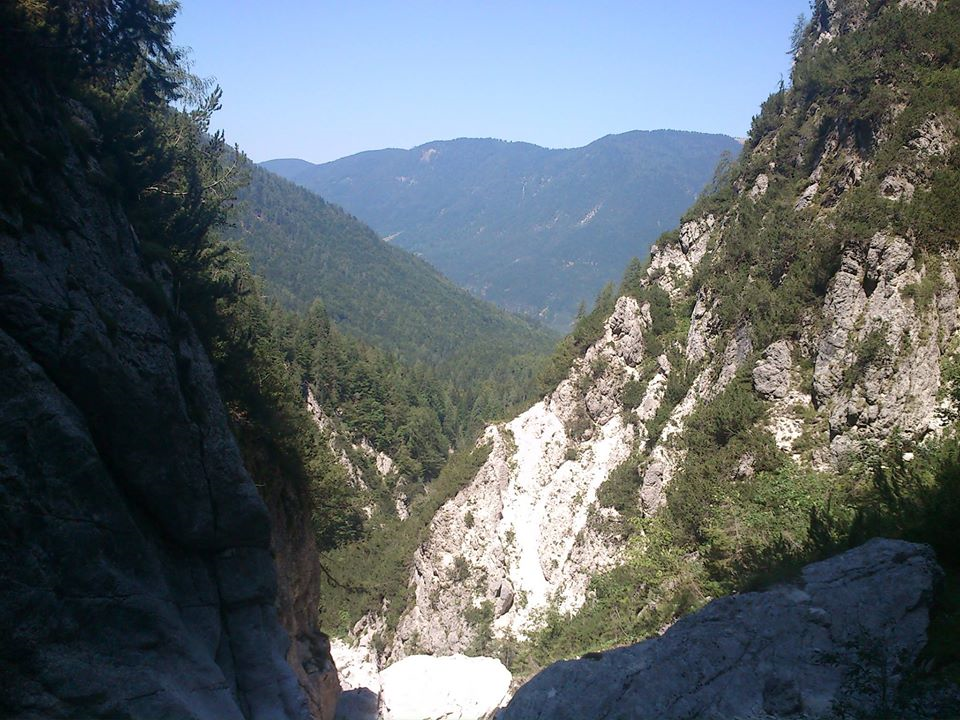
\includegraphics[height=6.5cm]{Pics/mountains.png}
\end{frame}

\begin{frame}[fragile]{Lightswitch in C\#}
\begin{lstlisting}[frame=shadowbox]
public class Lightswitch : MonoBehaviour {
  bool state;
  bool previousInput;
	
  void Update () {
    bool currentInput = Input.IsKeyDown(Keys.Space);
    if (!previousInput && currentInput) {
      state = !state;
      if(state)
        renderer.material.color = new Color(0, 0, 0);
      else 
        renderer.material.color = new Color(1, 1, 1);
    }
    previousInput = currentInput;
  }
}
\end{lstlisting}
\end{frame}

\begin{frame}[fragile]{Simple light-switch}
\begin{lstlisting}[frame=shadowbox]
world LightSwitch = {
  S : Sprite
  P : bool
  rule P = 
    when(IsKeyDown(Keys.Space))
    yield true
    yield false
    when(IsKeyUp(Keys.Space))
  rule S.Color = 
    yield Color.White
    when P
    yield Color.Black
    when P
}
\end{lstlisting}
\end{frame}

\begin{frame}[fragile]{Three state light-switch}
\begin{lstlisting}[frame=shadowbox]
world LightSwitch = {
  S : Sprite
  P : bool
  rule P = ...
  rule S.Color = 
    yield Color.Green
    when P
    yield Color.Orange
    when P
    yield Color.Red
    when P
}
\end{lstlisting}
\end{frame}

\begin{frame}[fragile]{Timed-on/off lightswitch}
\begin{lstlisting}[frame=shadowbox]
world LightSwitch = {
  S : Sprite
  rule S.Color = 
    yield Color.Green
    wait 2.0f<s>
    yield Color.Orange
    wait 1.0f<s>
    yield Color.Red
    wait 3.0f<s>
}
\end{lstlisting}
\end{frame}

\begin{frame}{Comparison with C\#}
\center
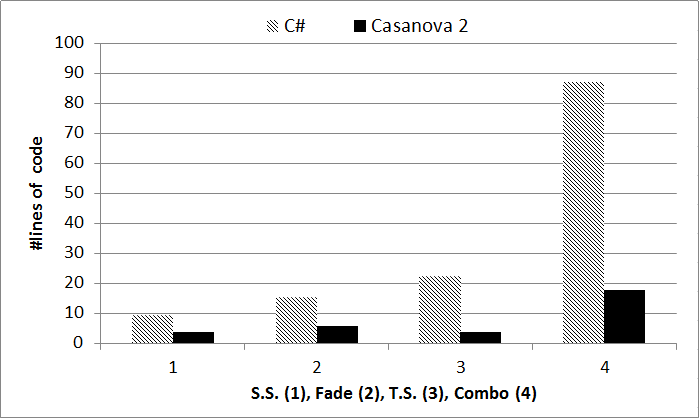
\includegraphics[height=6.0cm]{Pics/code_length_comparison.png}
\end{frame}

\begin{slide}{Casanova}{Readability}{
\item Programming languages are description tools
\item Their main goal is to \textit{tell another human what the machine should do} \cite{dijkstra1979programming}
\item Assessing the \textit{readability of a language} is crucial
}\end{slide}

\begin{slide}{Casanova}{Readability}{
\item Test: students\footnote{12 gamedev students, programming and design} read Casanova sources
\begin{table}[!t]
\caption{Feedback from students}
\label{students_feedback}
\centering
\begin{tabular}{|c||c|}
\hline
Syntax is unfamiliar at first & 3\\
\hline
Syntax is clear & 8\\
\hline
Indentation instead of parentheses is a downside & 2\\
\hline
List processing with queries is very effective & 1\\
\hline
Rules are a good abstraction for games & 2\\
\hline
\end{tabular}
\end{table}
}\end{slide}

\begin{slide}{Casanova}{Compiler structure}{
\item Parse
\item Analyse and optimize queries
\item Analyse and optimize \texttt{wait}s with state machines
\begin{itemize}
\item Event-system
\item Large \texttt{switch}-statement for each state machine
\end{itemize}
\item Generate main loop
\item Generate code
\begin{itemize}
\item Using the C\# syntax tree and Roslyn
\item Can also output C\# instead of binaries
\end{itemize}
}\end{slide}

\begin{slide}{Casanova}{Usage in practice}{
\item All nice and all, but does it work in reality?
\pause
\item Yup
\item DEMO (RTS game)
}\end{slide}

\begin{textslide}{Casanova}{Future endeavours}{
Networking in games
}\end{textslide}

\begin{frame}[fragile]{Networking}
\center
\begin{tabular}{| c | c |}
\hline
\begin{lstlisting}
local{
  rule X = 
    send(b)
    if b then
      yield receive()
    else
      wait 1.0f<s>
      send(c)
}
\end{lstlisting}
&
\begin{lstlisting}
remote{
  rule X = 
    let b = receive()
    if b then
      wait 1.0f<s>
      send(c)
    else
      yield receive()
}
\end{lstlisting}
\\
\hline
\end{tabular}
\end{frame}

\begin{slide}{Casanova}{Conclusions}{
\item Interaction negates termination, at least globally
\item Modern programming languages suffer from this
\item Need for better languages that handle time
\item Concept of ``do nothing'' at the language level
\begin{itemize}
\item High expressive power
\item Clean code
\item We argue results in a more pleasant ``game development experience''
\end{itemize}
}\end{slide}

\begin{frame}{That's it}
\center
\fontsize{18pt}{7.2}\selectfont
Thank you!
\end{frame}

\begin{frame}[allowframebreaks]
\frametitle{References}
\bibliographystyle{plain}
\bibliography{bibliography}
\end{frame}

\end{document}
